\section{算法设计}\label{algorithm}

\subsection{系统框架}
\subsection{基于点云的体渲染}


\subsubsection{体素采样}
我们使用一个隐式的SDF解码器$F_\theta$,一个隐式的语义解码器$G_\phi$(其中$\theta$和$\phi$为可优化的网络参数)和一个$N$维的存储在稀疏体素中的特征集合来表示一个场景。这些特征存储在每一个体素的8个顶点上,每一个特征都被相邻的体素共享,这些共享的特征可以优化体素边界上出现的伪影。

由于我们的体素是动态分配的,对于尚未进行建图的区域空间中存在大量的空白体素。因此,在空间中进行分层随机采样的方法会在无效的体素上浪费大量的算力。为了提高采样效率,对与当前点云帧中每一个被采样的点云,我们首先通过一个求交运算检查这条沿着从雷达位置到该点的光线是否穿过了任何有效体素。没有击中任何体素的采样点云会被剔除,因为其不会对渲染产生任何影响。考虑到复杂的大规模场景可能存在较远的边界,我们设置了一个采样点所能影响到的体素的最大数量$M_h$和最大的采样距离$D_max$。

如图\ref{shinemapping}所示,对于模拟出的光线,我们将以固定步长在从雷达位置到最大采样距离上进行等距采样。对于光线上的任意一个采样点,我们使用其处于的叶子节点上的8个$N$维特征进行三线性插值,得出该点的特征值。随后使用解码器进行解码。
\begin{figure}[htbp]
    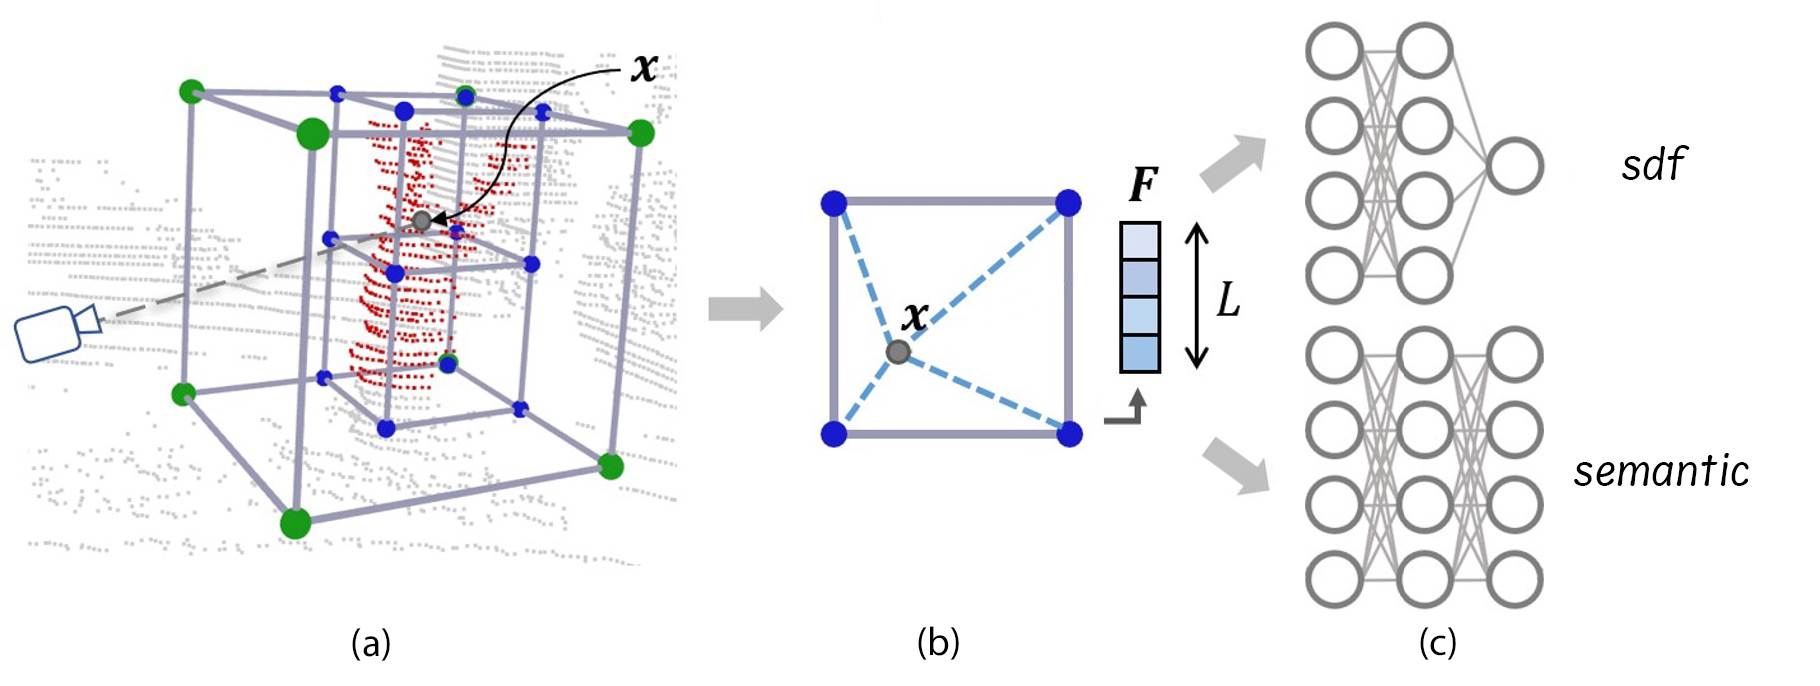
\includegraphics[scale = 0.3]{figures/shinemapping.png}
    \centering
    \caption{一次迭代中的正向传播步骤:首先模拟一条从激光雷达处发出的穿过被采样点云的光线,随后在光线上以固定步长采样(a),对于空间中每一个采样点,对叶子节点体素使用三线性插值计算出特征值(b),最后使用SDF解码器与语义解码器计算出最终结果(c)。}\label{shinemapping}
\end{figure}
\subsubsection{解码器}
如图\ref{shinemapping}所示,我们使用两个较浅的全连接层(MLP)$F_\theta$和$G_\phi$分别用来预测空间中任意一点的SDF值与语义信息。其中$F_\theta$的输出为一个一维数值,代表该点距离最近表面的距离;$G_\phi$的输出为一个$N_{sem}$维向量,其中$N_{sem}$表示语义标签种类的个数。该向量在推理时会被执行一次argmax函数得到最终语义标签的索引。
\subsubsection{隐式表面渲染}
相较于原始NeRF中使用MLP预测空间中任意一点的体密度,也就是占据概率,SDF能更好的表达几何信息,这也是为什么可以将其用于光线追踪中等任务中,因此我们在训练中直接回归SDF值。下列渲染公式表示了我们如何从嵌套在体素中的特征中获得该处点云最终的深度$D$和语义向量$\mathbf{S}$。假设我们在一条光线上采样$N$个点:
\begin{equation}
    s_i=F_\theta(\mbox{TriLerp}(T_i\mathbf{p}_i,\mathbf{e})),
\end{equation}
\begin{equation}
    \mathbf{S}_i=G_\phi(\mbox{TriLerp}(T_i\mathbf{p}_i,\mathbf{e})),
\end{equation}
\begin{equation}
    w_i=\mathbf{\sigma}(\frac{s_i}{tr})\cdot\mathbf{\sigma}(-\frac{s_i}{tr})
\end{equation}
\begin{equation}
    \mathbf{S} = \frac{1}{\sum_{j=0}^{N-1}w_j}\sum_{i=0}^{N-1}w_i\cdot\mathbf{S}_i
\end{equation}
\begin{equation}
    D = \frac{1}{\sum_{j=0}^{N-1}w_j}\sum_{i=0}^{N-1}w_i\cdot d_i
\end{equation}
其中$T_i$表示当前帧激光雷达的位置, $\mathbf{p}_i$表示该点在体素中的相对坐标,$\mbox{TriLerp}(\cdot , \cdot)$表示三线性插值函数, $\mathbf{e}$表示存储在体素中的特征。$F_\theta\mbox{和}G_\phi$分别为带可优化网络参数的解码器。为了计算每一个采样点的权重$w_i$, 我们使用sigmoid函数$\mathbf{\sigma}$计算两次这个点的sdf值$s_i$与先前设置的截断距离$tr$的比值的正负值,并相乘。我们使用该权重对每个采样点的语义向量$\mathbf{S}_i$进行加权积分得到最终结果$\mathbf{S}$。同样的,为了得到深度值,我们对这条光线上每一个采点的深度进行积分,其中$d_i$为第$i$个采样点的深度。
\subsection{建图}
\subsubsection{地图优化}
\cite{adam}
\subsubsection{动态体素管理}
\subsubsection{全局建图与关键帧选择}
\begin{figure}[htbp]
    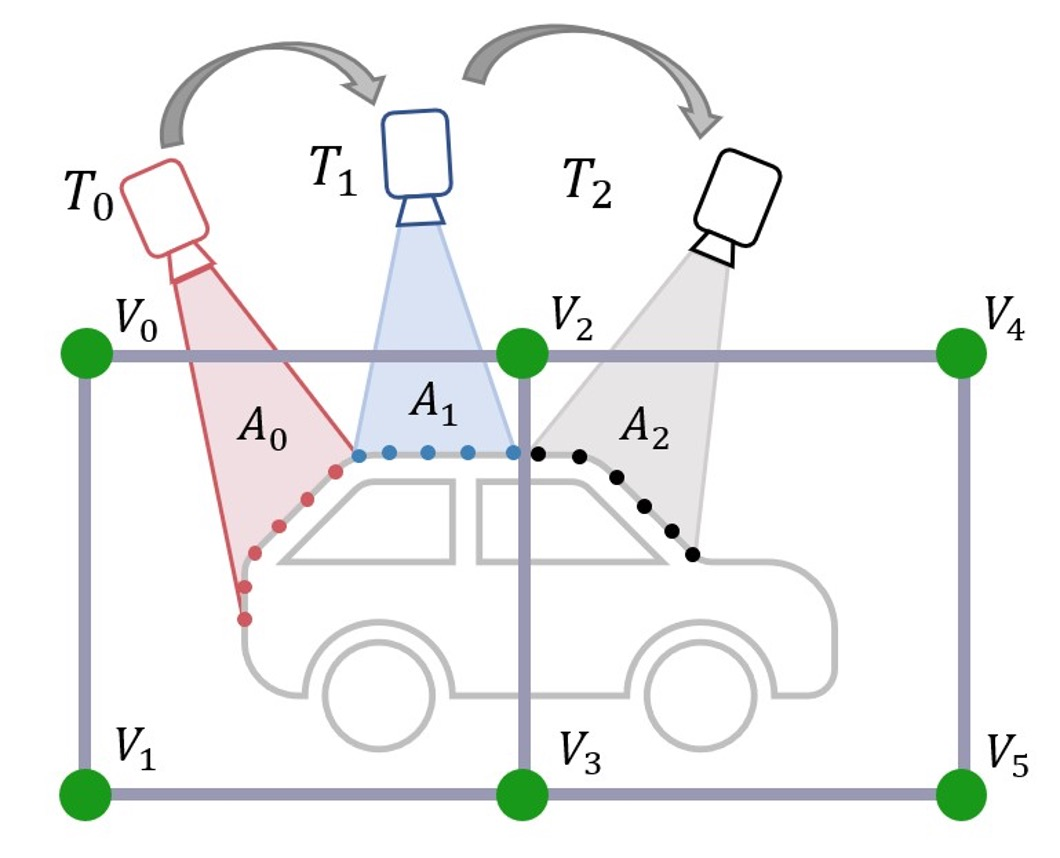
\includegraphics[scale = 0.2]{figures/forgetting.jpg}
    \centering
    \caption{在特征网格中进行增量建图时发生遗忘问题的例子} \label{forgetting}
\end{figure}
将大规模场景以增量建图方法编码会受到灾难性遗忘(Catastrophic Forgetting)问题的限制。如图\ref{forgetting}所示,在每一帧中($T_0, T_1$和$T_2$),系统仅能观察到环境的部分信息。在增量建图中的第$T_0$帧,我们使用从区域A0获取到的信息优化存储在网格中的特征$V_0, V_1, V_2$和$V_3$,因此$V_0, V_1, V_2$和$V_3$这4个特征将能较精确的表示区域A0的几何信息。然而当相机向前移动,使用T1帧更新$V_0, V_1, V_2$和$V_3$的特征时,网络将仅关注生成$A_1$时的损失,不再关注$A_0$区域的表现。当相机进一步移动至$T_2$帧时,$V_2$和$V_3$中的特征将再次被更新,但我们无法保证不会影响到$A_0$和$A_1$区域的建图精度。这就是遗忘问题发生的原因。

为了解决灾难性遗忘问题,我们记录关键帧对网络进行重复训练。我们维护了一个关键帧集合K,使用Vox-Fusion中的策略,即八叉树体素结构的变化量决定何时插入关键帧:每当新的一帧出现时,体素管理系统会执行求交运算得出需要新分配体素的数量$N_c$,而当前存储的体素数量为$N_o$,当两者比值$p_{kf}=N_c/N_o$大于某一阈值时,当前帧将被插入关键帧集合。某种极端情况下,当相机移动处于一个循环状态时,可能出现只有极少体素或没有体素被新分配,导致永远没有关键帧被插入。因此,我们也设定了相邻关键帧的最大距离,例如,当之前的$N$帧都不是关键帧时,自动插入一个关键帧。

在第全局建图线程中,我们使用一个窗口从关键帧集合$K$中随机选取$N_{kf}$个关键帧作为优化目标对地图进行全局优化,与增量建图线程同步进行。
